\documentclass[11pt]{article}
\usepackage[utf8]{inputenc}	% Para caracteres en español
\usepackage{amsmath,amsthm,amsfonts,amssymb,amscd}
\usepackage{multirow,booktabs}
\usepackage[table]{xcolor}
\usepackage{fullpage}
\usepackage{lastpage}
\usepackage{enumitem}
\usepackage{fancyhdr}
\usepackage{mathrsfs}
\usepackage{wrapfig}
\usepackage{setspace}
\usepackage{calc}
\usepackage{multicol}
\usepackage{cancel}
\usepackage[retainorgcmds]{IEEEtrantools}
\usepackage[margin=1cm]{geometry}
\usepackage{amsmath}
\newlength{\tabcont}
\setlength{\parindent}{0.0in}
\setlength{\parskip}{0.05in}
\usepackage{empheq}
\usepackage{framed}
\usepackage[most]{tcolorbox}
\usepackage{xcolor}
\usepackage{graphicx}
\usepackage{listings}
% -- Basic formatting
\usepackage[utf8]{inputenc}
\usepackage[english]{babel}
\usepackage{times}
\usepackage{caption}
\usepackage{subcaption}
\usepackage{placeins}
\setlength{\parindent}{0pt}
\usepackage{indentfirst}% -- Defining colors:
\usepackage[dvipsnames]{xcolor}
\definecolor{codegreen}{rgb}{0,0.6,0}
\definecolor{codegray}{rgb}{0.5,0.5,0.5}
\definecolor{codepurple}{rgb}{0.58,0,0.82}
\definecolor{backcolour}{rgb}{0.95,0.95,0.92}% Definig a custom style:
\lstdefinestyle{mystyle}{
    backgroundcolor=\color{backcolour},   
    commentstyle=\color{codepurple},
    keywordstyle=\color{NavyBlue},
    numberstyle=\tiny\color{codegray},
    stringstyle=\color{codepurple},
    basicstyle=\ttfamily\footnotesize\bfseries,
    breakatwhitespace=false,         
    breaklines=true,                 
    captionpos=t,                    
    keepspaces=true,                 
    numbers=left,                    
    numbersep=5pt,                  
    showspaces=false,                
    showstringspaces=false,
    showtabs=false,                  
    tabsize=2
}% -- Setting up the custom style:
\lstset{style=mystyle}
\lstset{
  style=mystyle,
  framexleftmargin=3.5mm,
  rulesepcolor=\color{black},
  linewidth=0.6\linewidth,
  xleftmargin=12pt,
  aboveskip=12pt,
  belowskip=12pt
}
\colorlet{shadecolor}{orange!15}
\parindent 0in
\parskip 1pt
\geometry{margin=1in, headsep=0.25in}
\theoremstyle{definition}
\newtheorem{defn}{Definition}
\newtheorem{reg}{Rule}
\newtheorem{exer}{Exercise}
\newtheorem{note}{Note}
\graphicspath{ {./images/} }
\begin{document}
\setcounter{section}{0}
\title{MIE223 Lecture Notes}

\thispagestyle{empty}

\begin{center}
{\LARGE \bf Fairness and Bias}\\
{\large MIE223}\\
Winter 2025
\end{center}
\section{Introduction to Fairness and Bias}
\subsection{MIT Study on Racial/Gender Discrimination in Image Classifiers}
\begin{itemize}
    \item MIT Project known as Gender Shades
    \begin{itemize}
        \item Examined facial recognition algorithms from Microsoft and IBM:
        \item Did poorly on underrepresented groups (e.g. black females)
    \end{itemize}
\end{itemize}
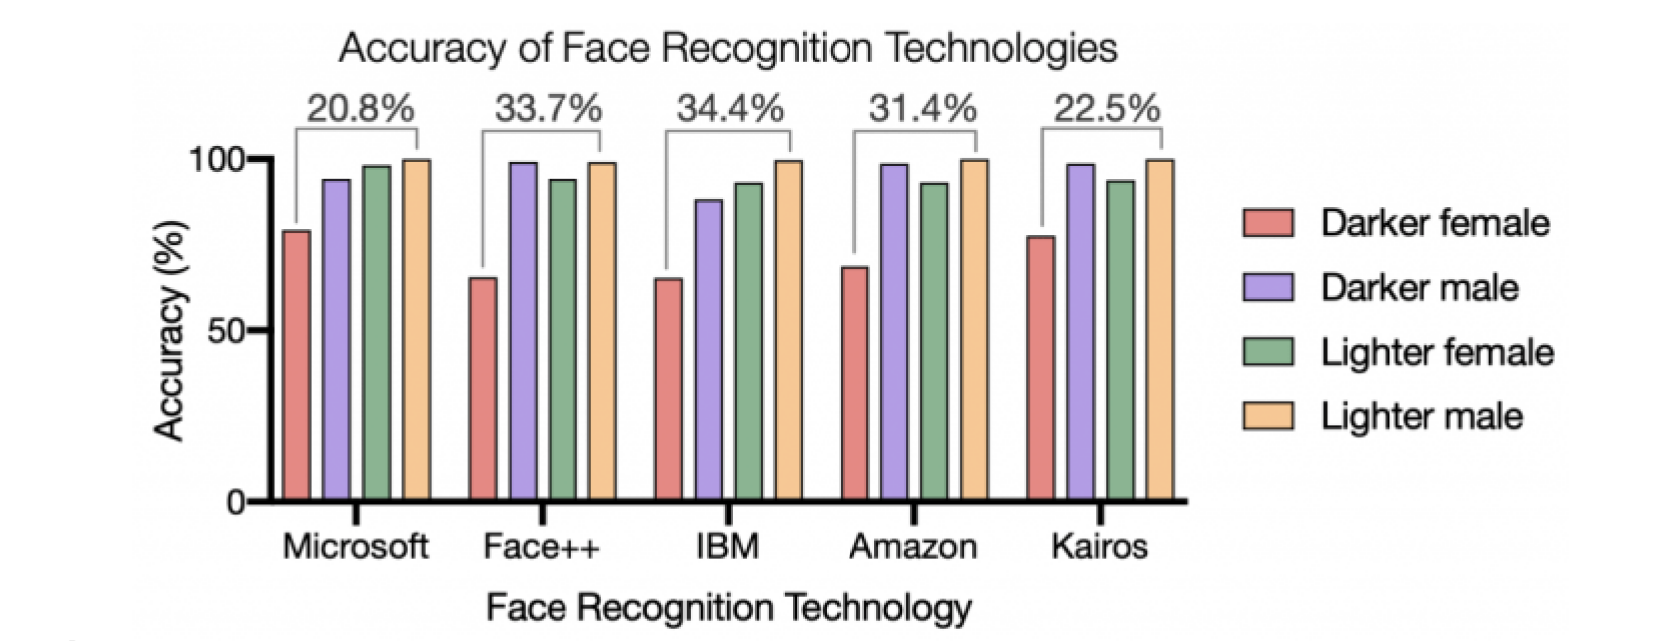
\includegraphics[width = \textwidth]{1.png}
\subsection{Data is Full of Biases}
Representation and Collection Bias
\begin{itemize}
    \item The data is not representative of the population distribution it is intended to serve
    \begin{itemize}
        \item Critical in medicine
    \end{itemize}
    \item The data has insufficient representation of minority groups
\end{itemize}

Measurement and Historical Bias
\begin{itemize}
    \item What you measure is misaligned with
    use case, or biased from historical data
    \begin{itemize}
        \item E.g., using historical loan decisions to
        inform future decisions
    \end{itemize}
\end{itemize}

Aggregation bias
\begin{itemize}
    \item Effect for a group can be reversed
    when looking at data in aggregate
\end{itemize}

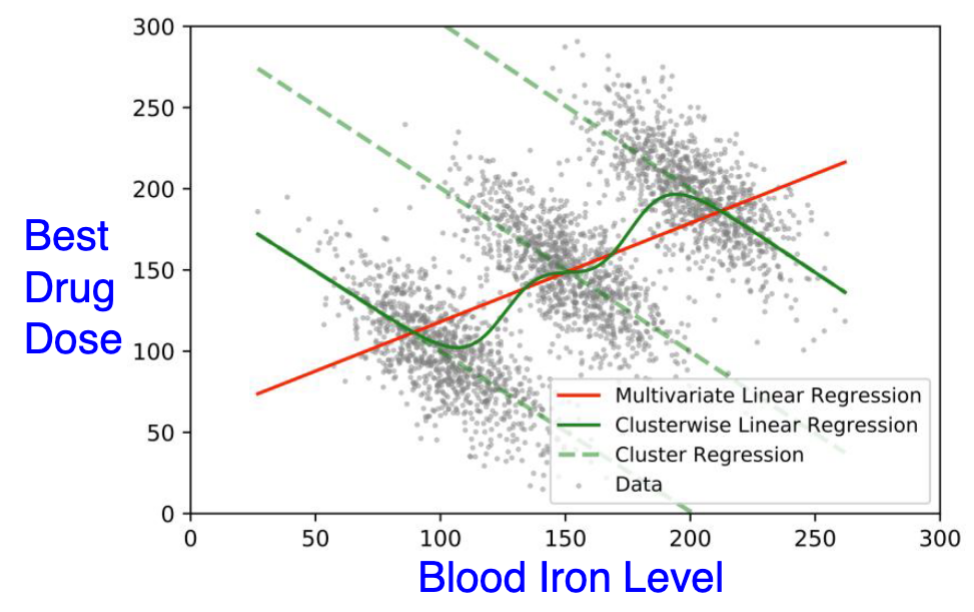
\includegraphics[width = \textwidth/2]{2.png}

This data is multimodal. Gaussian means unimodal, so be careful
applying unimodal tools to multimodal data.
If you ignore modes, you get the red line rather
than the green line.

\subsection{Group and Individual Fairness}
Much research on fairness aims to ensure “fair treatment” = parity

Group Fairness
\begin{itemize}
    \item Achieve “parity” (equality) across protected and advantaged groups
    \item Groups usually determined by demographic attribute
    \begin{itemize}
        \item e.g., {Caucasian, non-Caucasian}, {Male, non-Male}
    \end{itemize}
\end{itemize}

Individual Fairness
\begin{itemize}
    \item Similar individuals should have similar predictions / outcomes
    \item Requires measure of similarity between individuals
    \begin{itemize}
        \item e.g., Euclidean or cosine similarity between demographic feature vectors
    \end{itemize}
\end{itemize}

\subsection{Group and Individual Fairness for Classification}
Classification: predicting a discrete label, e.g., {parole, no parole}

\begin{itemize}
    \item Group Fairness:
    \begin{itemize}
        \item Fairness in Treatment: should not consider sensitive/protected attribute (e.g., gender, race, age)
        \begin{itemize}
            \item But other attributes may be correlated with sensitive ones!
        \end{itemize}
        \item Fairness in Impact: classification outcome should be balanced across groups
        \begin{itemize}
            \item E.g., false positive rate for each group should be the same
        \end{itemize}
    \end{itemize}
    \item Individual Fairness:
    \begin{itemize}
        \item Enforce similar individuals to receive similar outputs (or distributions)
        \begin{itemize}
            \item Requires a similarity function over sensitive attributes
        \end{itemize}
    \end{itemize}
\end{itemize}

\subsection{On the chalkboard}
Given your grades (vectorized) in previous courses, what letter grade will you get in this course?
Your past history helps predict your future performance.
You can regress directly to the grade, whereas classification goes to letter grades {A,B,C,D,F}
Focusing on binary classification {P, NP}:
\begin{itemize}
    \item True Positive (TP): predicted positive and actually positive
    \item True Negative (TN): predicted negative and actually negative
    \item False Positive (FP): predicted positive and actually negative
    \item False Negative (FN): predicted negative and actually positive
\end{itemize}
\begin{equation}
    \text{Accuracy} = \frac{TP + TN}{TP + TN + FP + FN}
\end{equation}
\begin{equation}
    \text{True Positive Rate (TPR)} = \frac{TP}{TP + FN}
\end{equation}
\begin{equation}
    \text{False Positive Rate (FPR)} = \frac{FP}{FP + TN}
\end{equation}
\begin{equation}
    \text{False Discovery Rate (FDR)} = \frac{FP}{TP + FP}
\end{equation}
\begin{equation}
    \text{True Negative Rate (TNR)} = \frac{TN}{TN + FP}
\end{equation}
\begin{equation}
    \text{False Negative Rate (FNR)} = \frac{FN}{TP + FN}
\end{equation}
\begin{equation}
    \text{Precision} = \frac{TP}{TP + FP}
\end{equation}
\begin{equation}
    \text{Recall} = \frac{TP}{TP + FN}
\end{equation}
\begin{equation}
    \text{F1 Score} = 2 \cdot \frac{\text{Precision} \cdot \text{Recall}}{\text{Precision} + \text{Recall}}
\end{equation}
\begin{equation}
    \text{F2 Score} = (1 + 2) \cdot \frac{\text{Precision} \cdot \text{Recall}}{\text{Precision} + 2 \cdot \text{Recall}}
\end{equation}
\begin{equation}
    \text{F0.5 Score} = (1 + 0.5) \cdot \frac{\text{Precision} \cdot \text{Recall}}{\text{Precision} + 0.5 \cdot \text{Recall}}
\end{equation}

Contingency table is a 2x2 table that summarizes the performance of a classification model
Multiclass classification uses a confusion matrix

\subsection{Achieving Parity}
What types of parity in binary classification can we aim for?

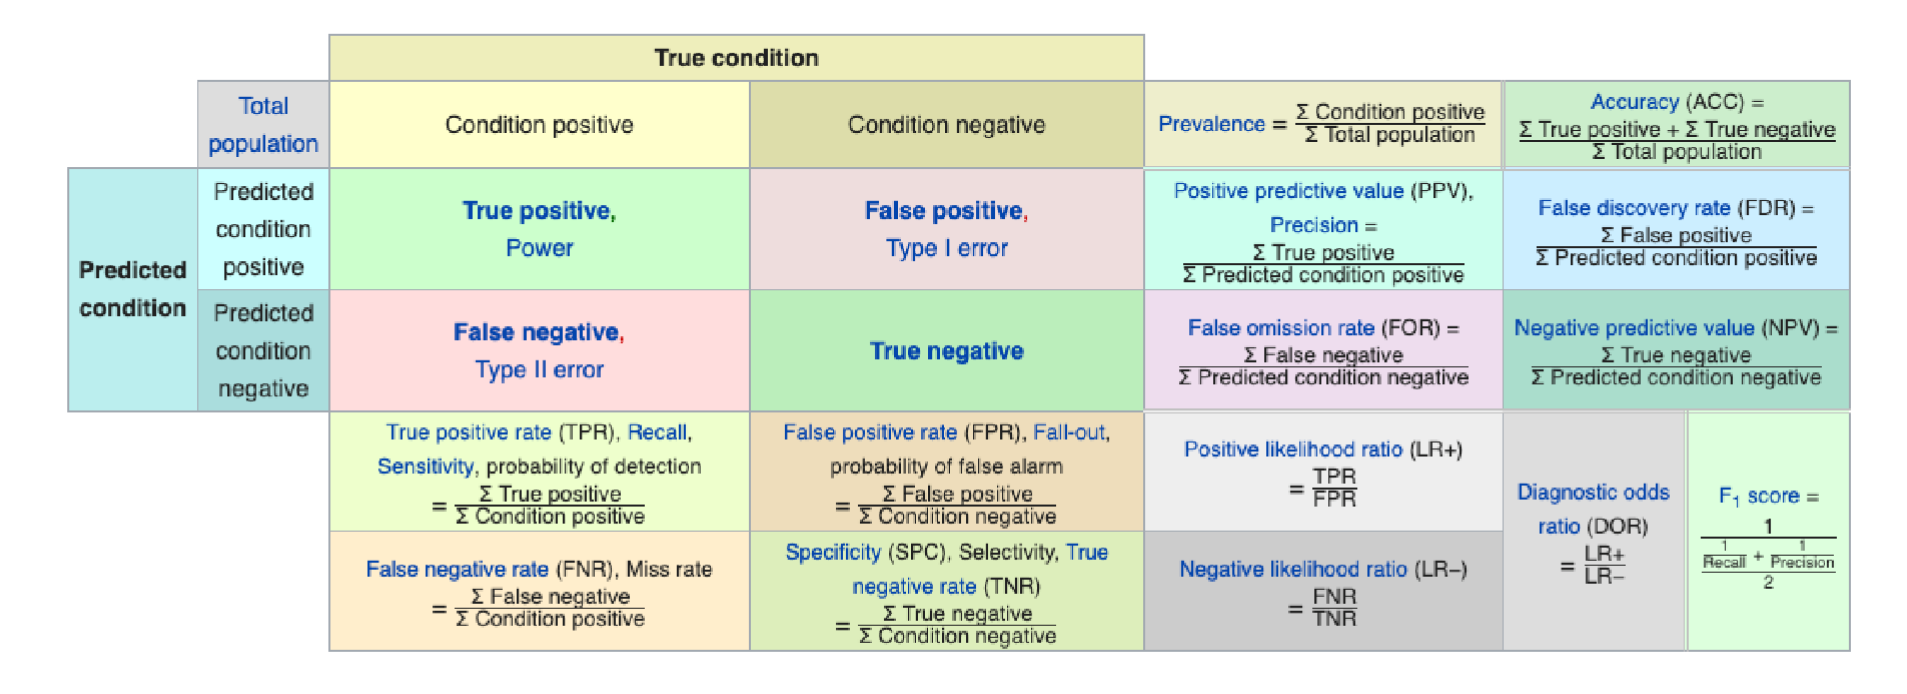
\includegraphics[width=\textwidth]{3.png}

What types of parity can we aim for in impact fairness?
\begin{itemize}
    \item Demographic / statistical parity (predicted outcome only)
    \begin{itemize}
        \item Different groups get same positive classification rates
        \begin{itemize}
            \item E.g., same admission rate regardless of economic status
        \end{itemize}
    \end{itemize}
    \item Parity in errors (consider predicted and actual outcome)
    \begin{itemize}
        \item Different groups have different classification rates
        \item But we constrain the error rates (Accuracy, TPR, FPR, FDR, ...)
    \end{itemize}
\end{itemize}

\section{Can we have all desired Parities at once?}
No

\subsection{Incompatibility Between Fairness Metrics}
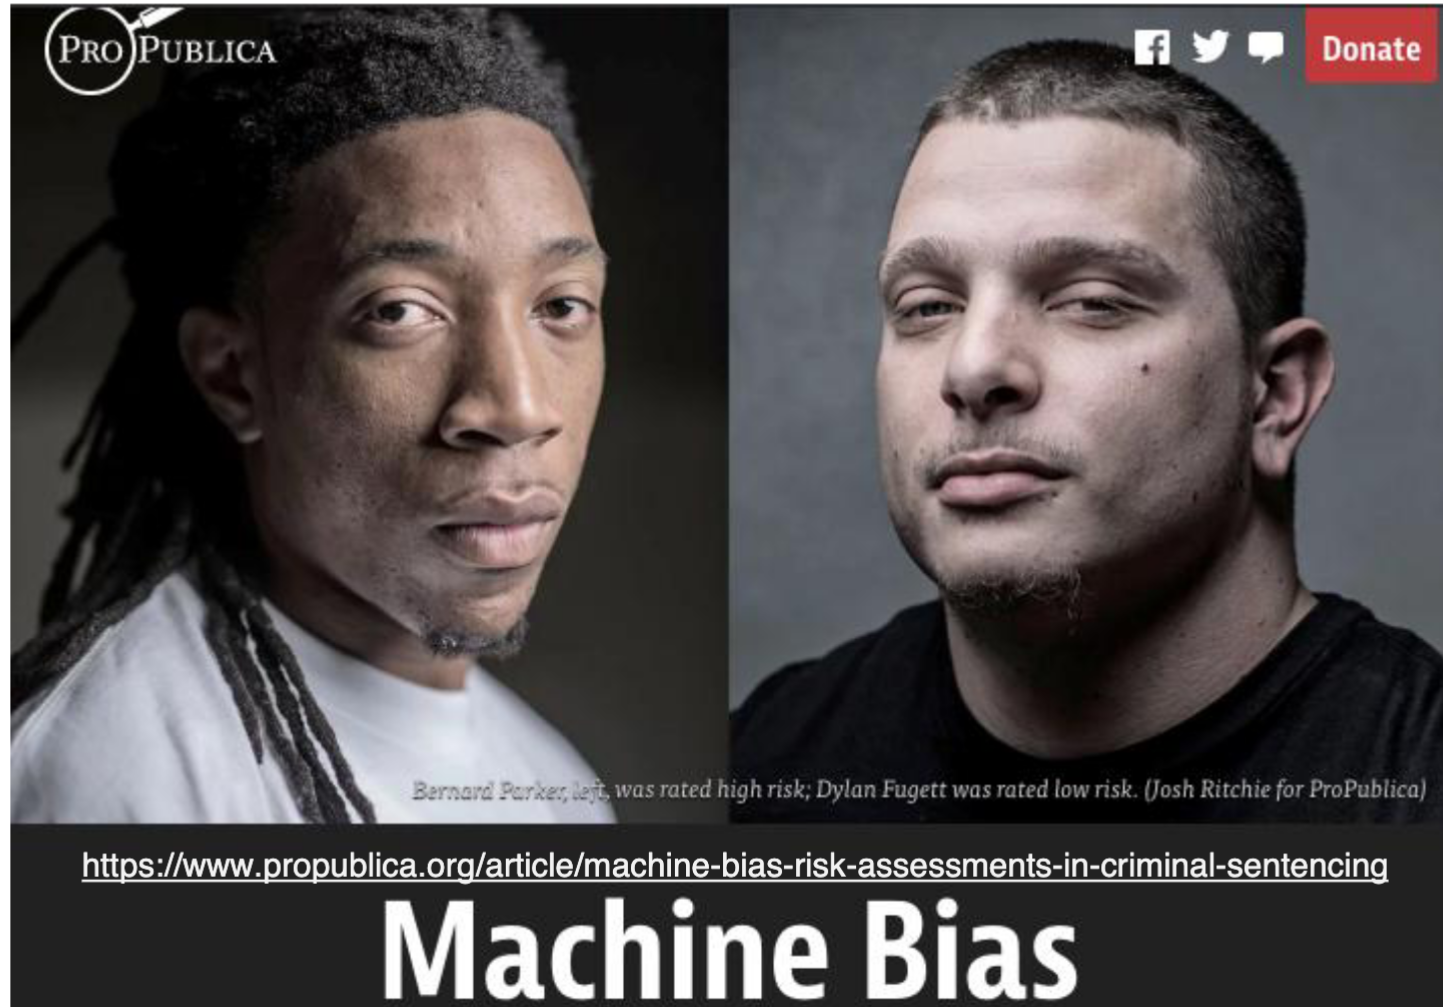
\includegraphics[width=\textwidth/2]{4.png}

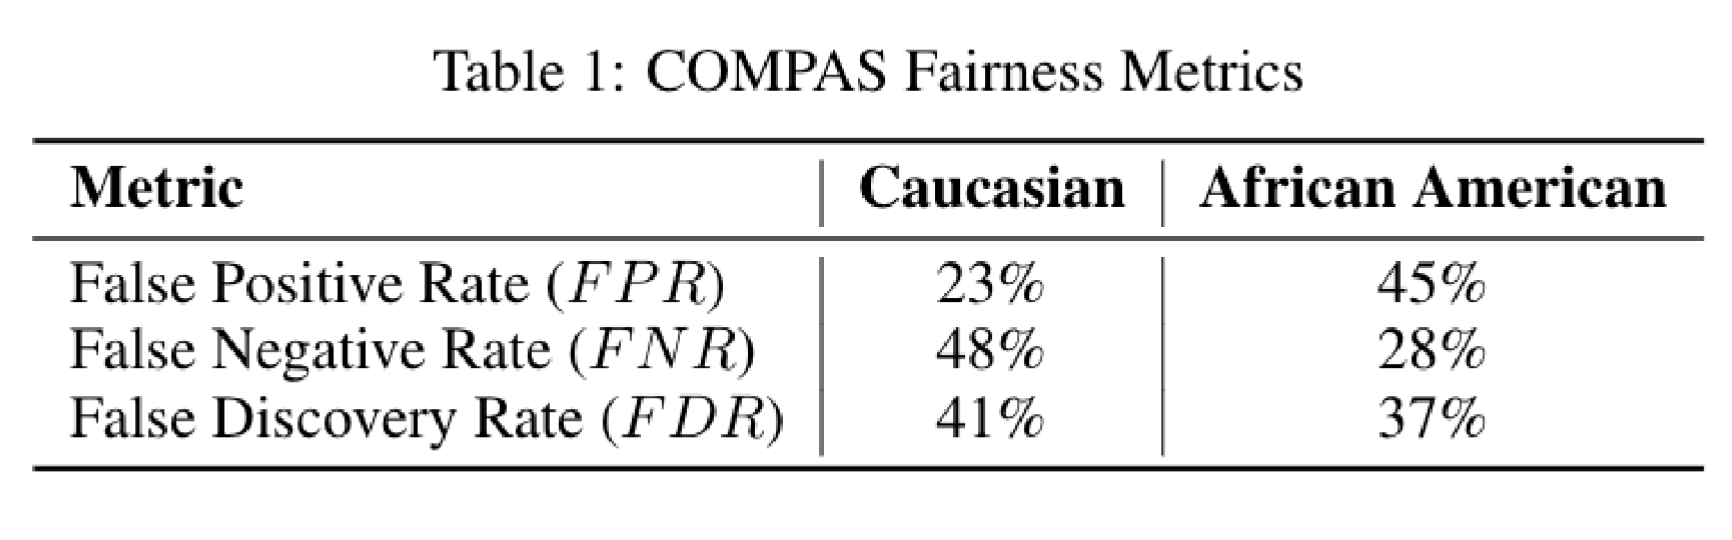
\includegraphics[width=\textwidth/2]{5.png}

ProPublica identified considerable disparities:
\begin{itemize}
    \item The algorithm was twice as likely to incorrectly predict black individuals were
    at high risk of recidivating (FPR)
    \item It was also nearly twice as likely to incorrectly predict white individuals were
    at low risk of recidivating (FNR)
\end{itemize}
However, the creator of the algorithm pointed out that the algorithm is well-
balanced across races on precision (equivalently, FDR), claiming this is the
correct measure of fairness in this context.

\begin{itemize}
    \item Who is right?
    \item Is the COMPAS algorithm biased?
    \item Can’t the algorithm achieve both
    measures of fairness at the same time?
\end{itemize}

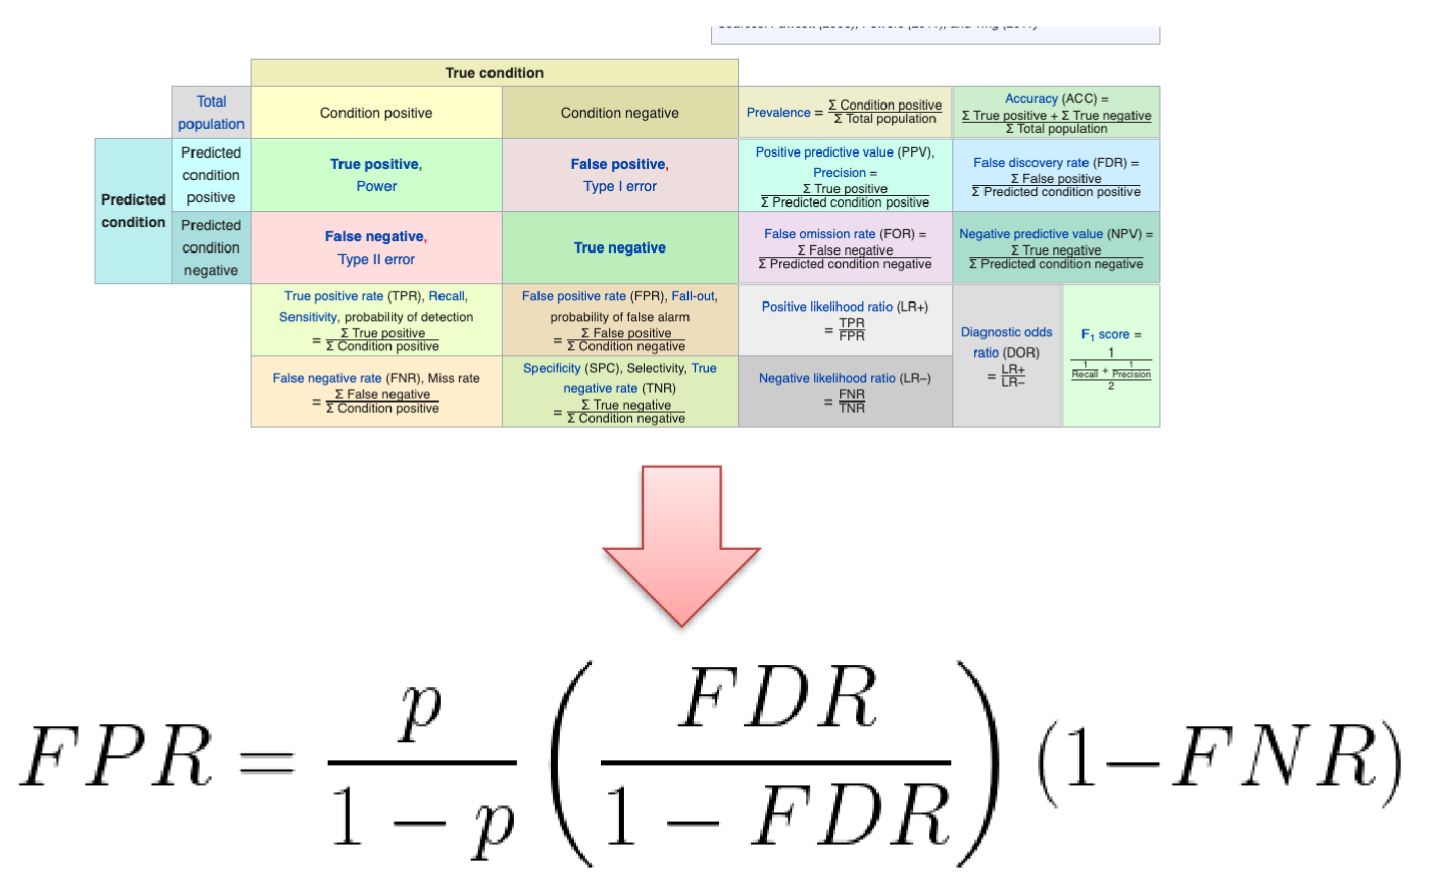
\includegraphics[width=\textwidth/2]{6.png}
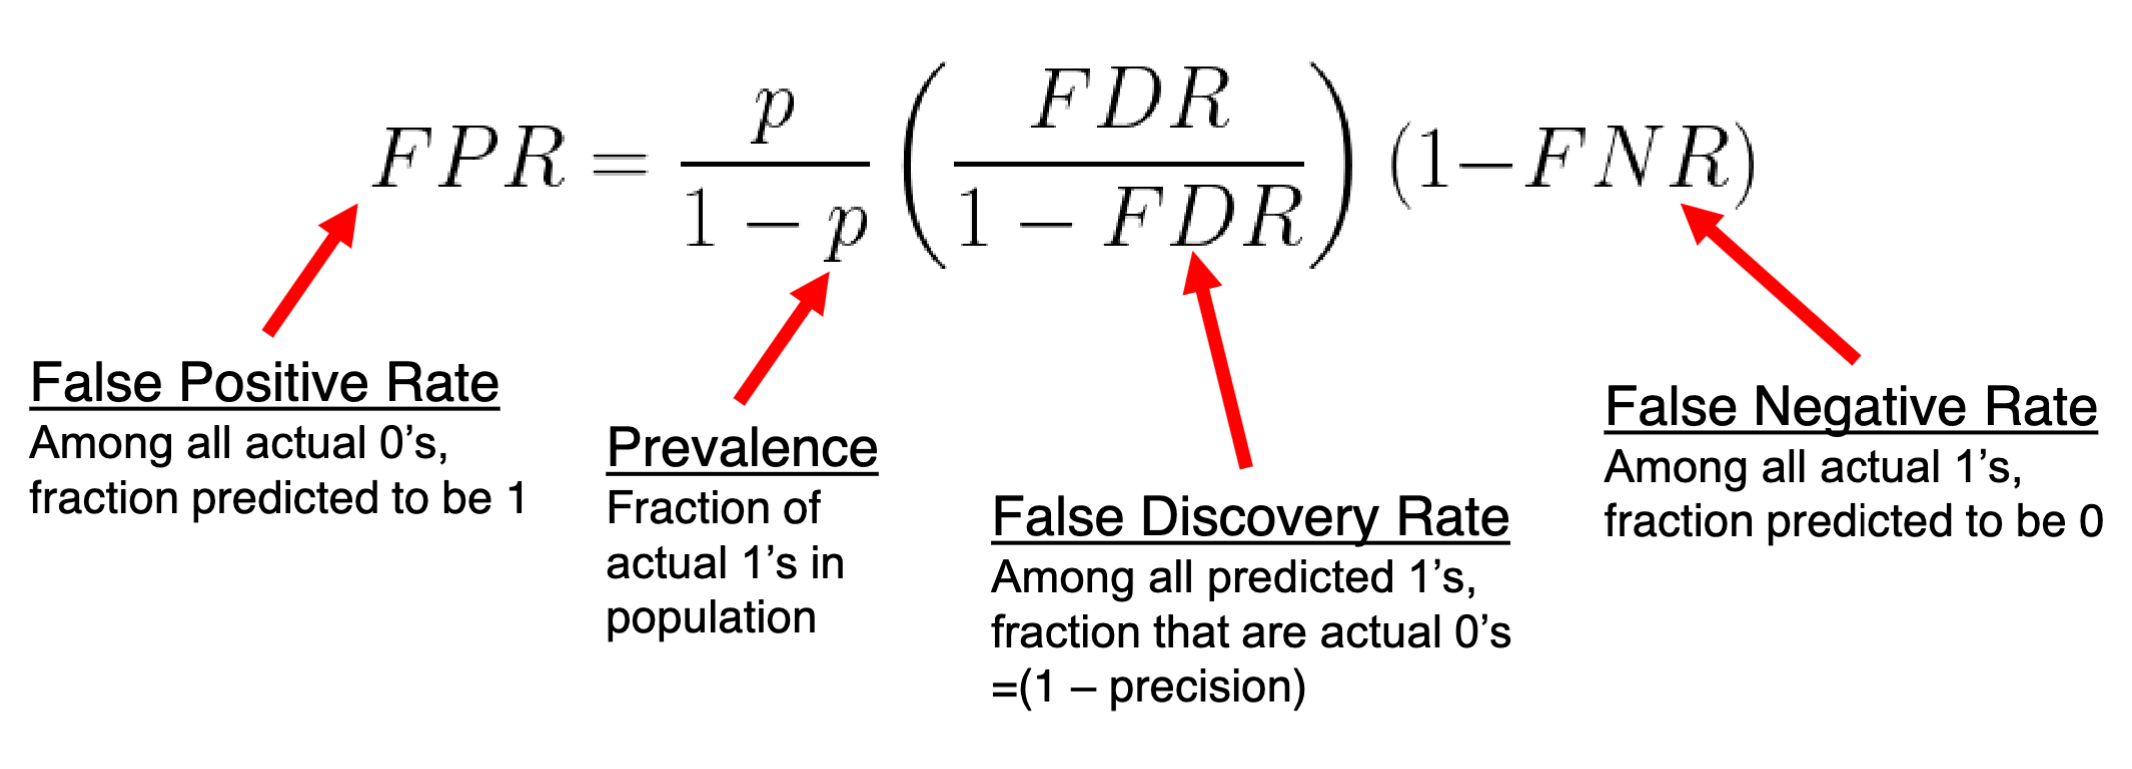
\includegraphics[width=\textwidth/2]{7.png}
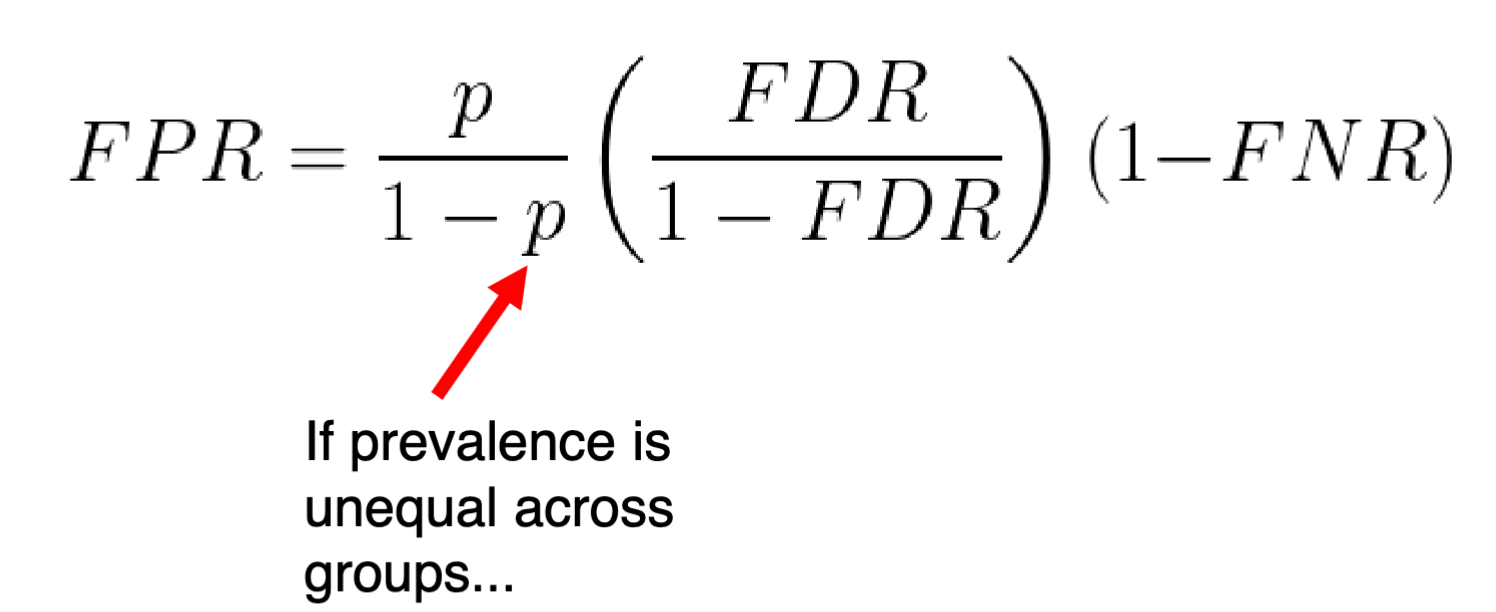
\includegraphics[width=\textwidth/2]{8.png}
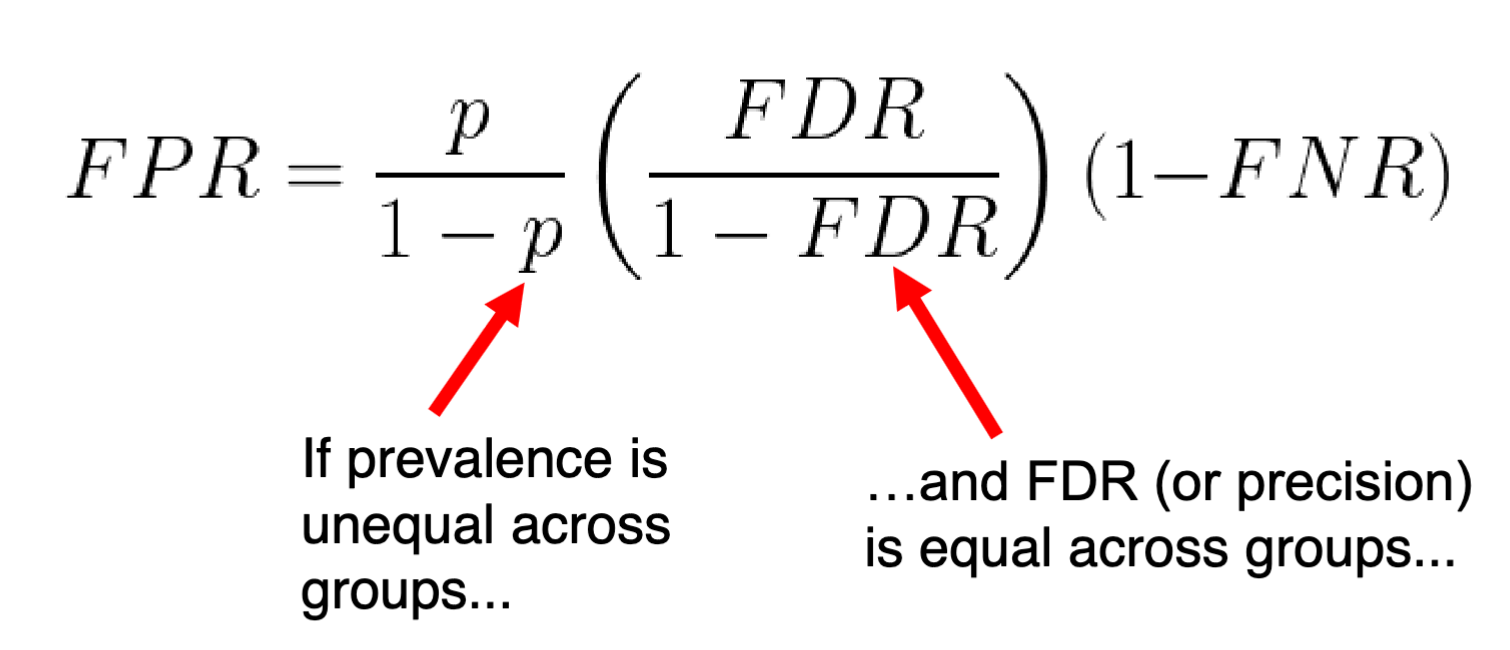
\includegraphics[width=\textwidth/2]{9.png}
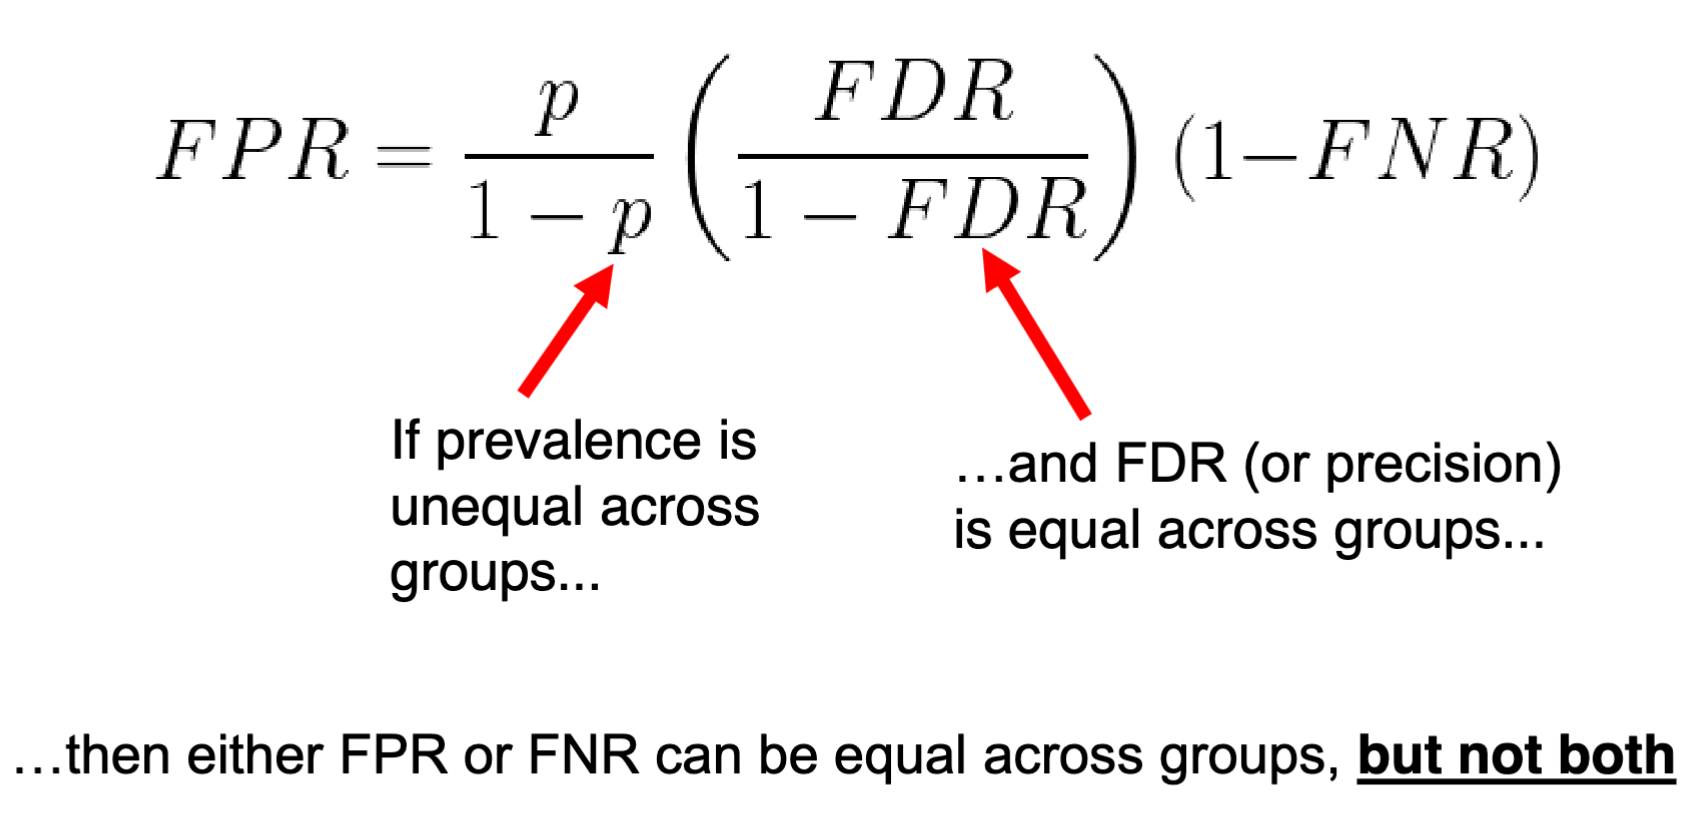
\includegraphics[width=\textwidth/2]{10.png}

\subsection{So... what does this mean?}
Sadly, no... we can’t have it all!
But this also doesn’t mean fairness is unachievable or
we shouldn’t bother.
Instead, it means we have to carefully consider and
choose the appropriate fairness metrics for our
context

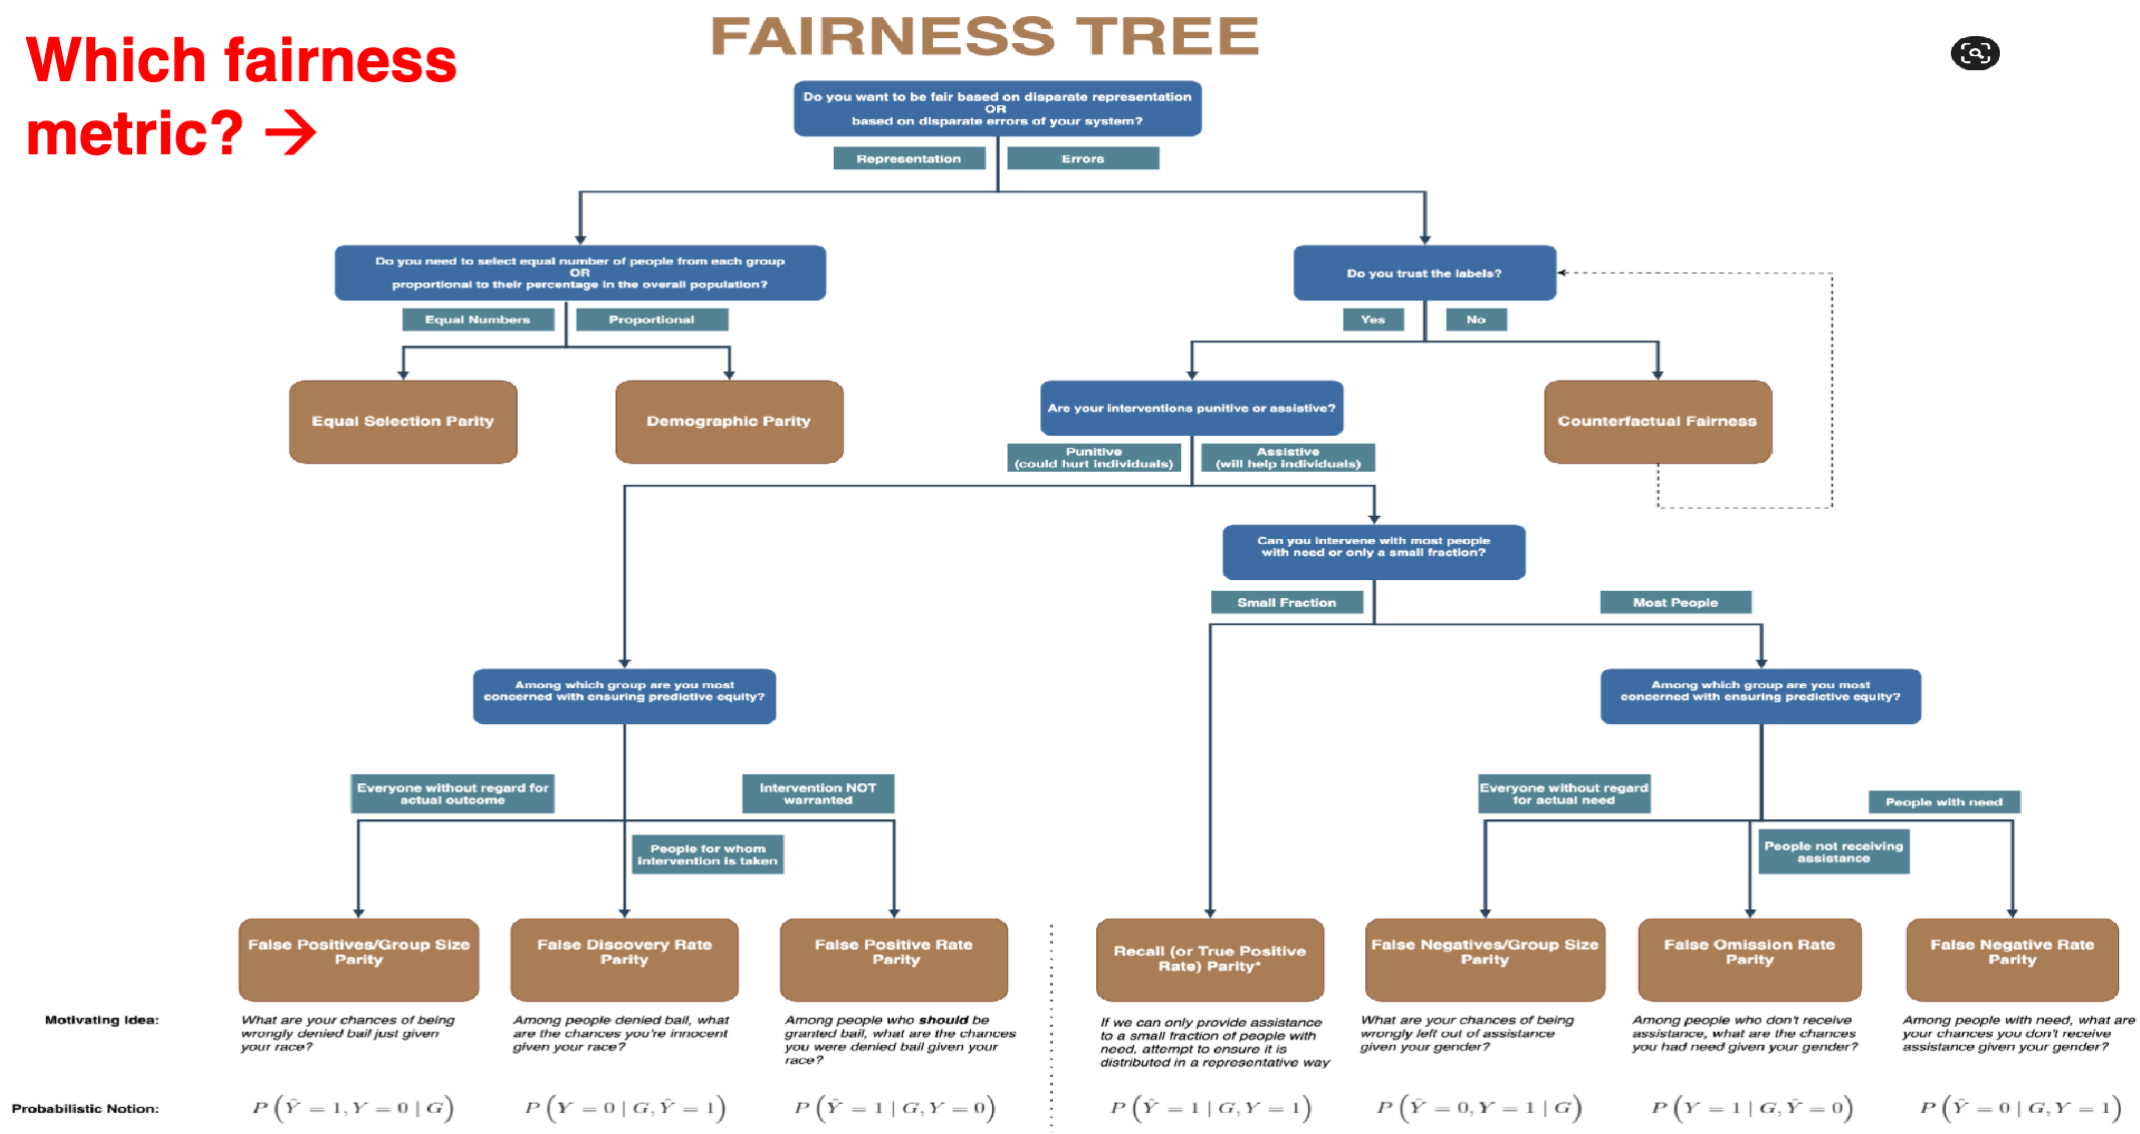
\includegraphics[width=\textwidth]{11.png}
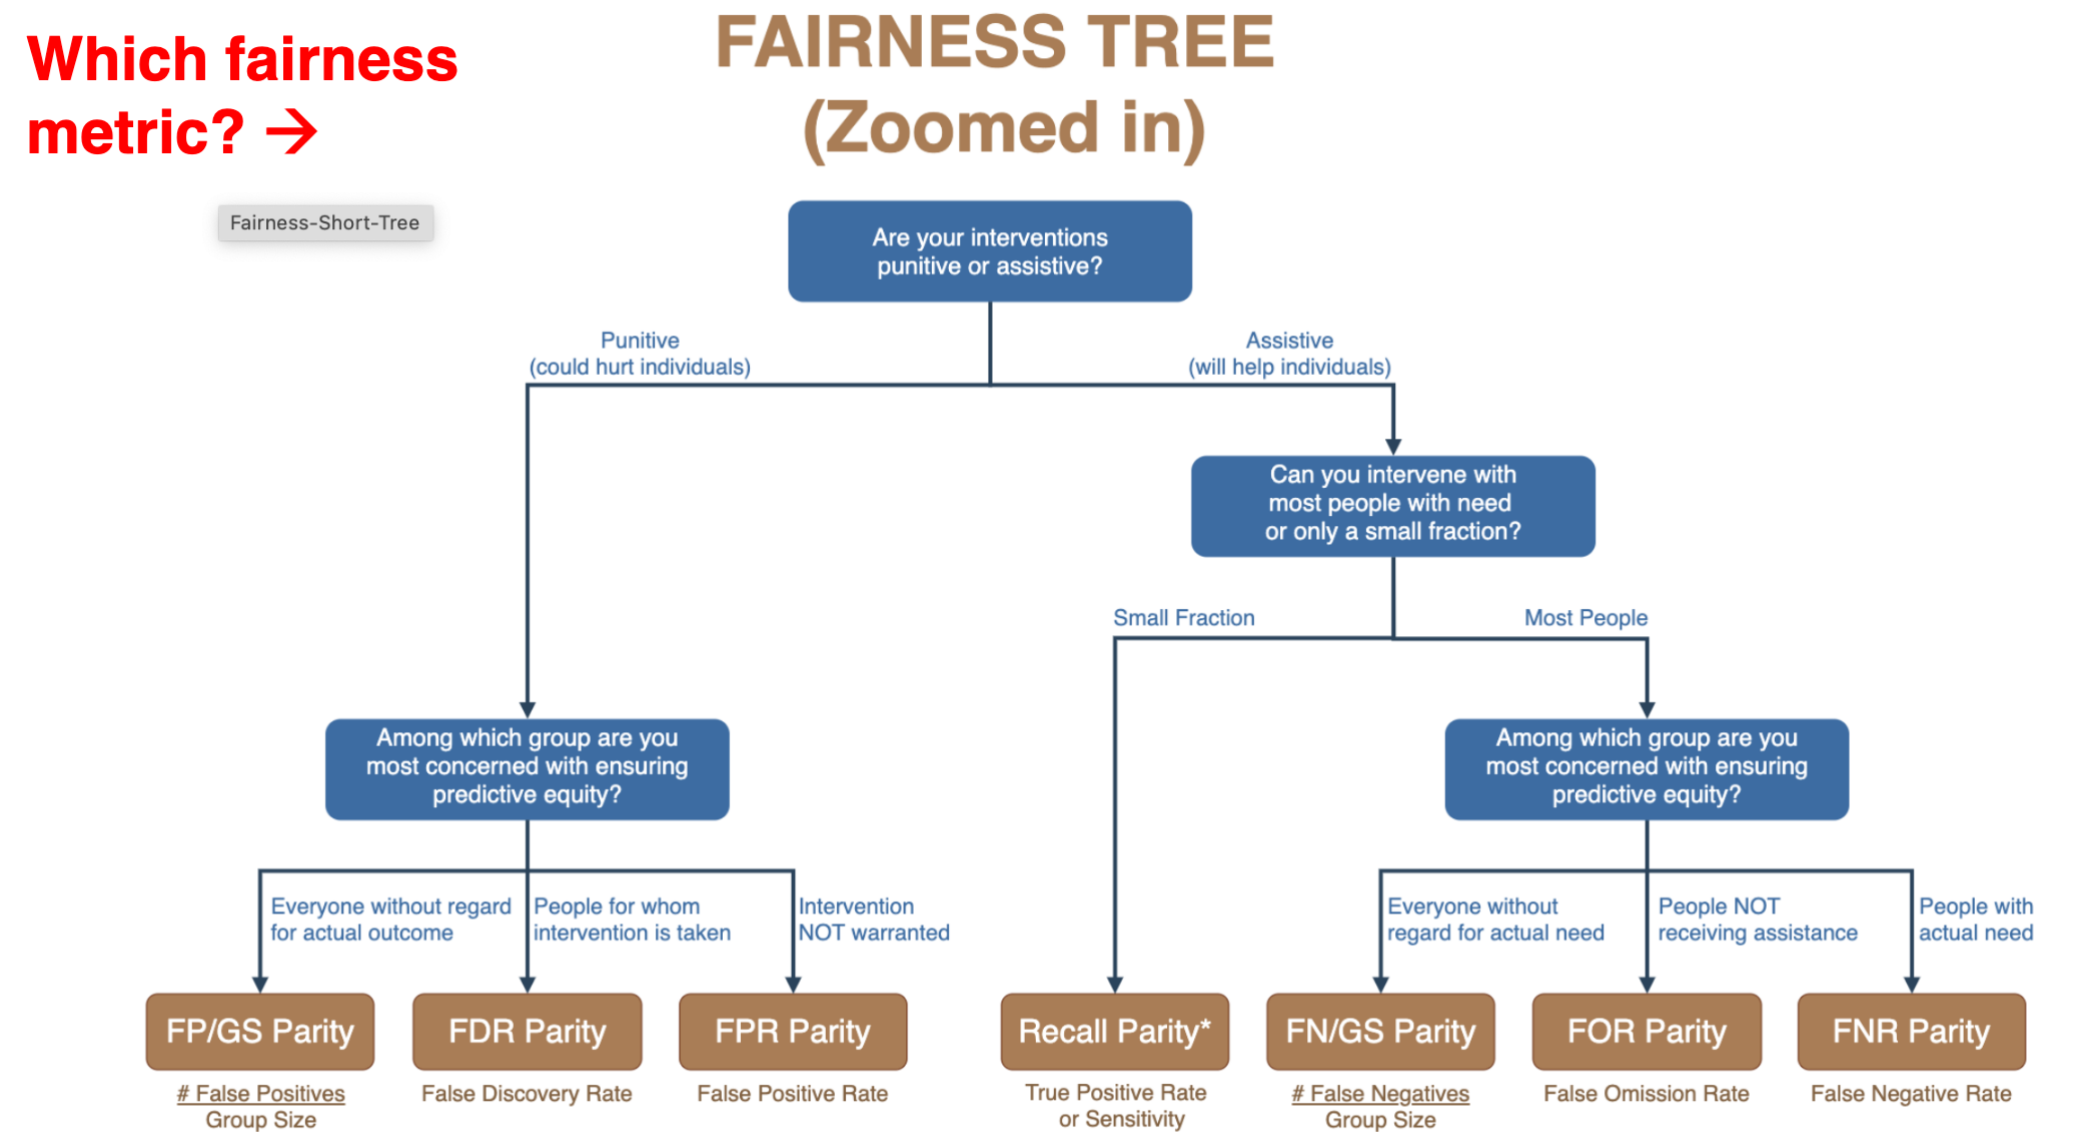
\includegraphics[width=\textwidth]{12.png}

\section{Working with Data Collected from
Humans (e.g., Surveys)}
Something you will likely do in your career
Beware of many biases that can occur!
(with potentially global impact: 2016 US election

\subsection{Survey Methodology and Bias Prevention}
\begin{itemize}
    \item Survey Sampling and Bias:
    \item Question Design and Cognitive Biases:
\end{itemize}

\end{document}